\section{Motivation}\label{sec:motivation}
Design decisions are crucial for shaping software architecture and defining its structure, organization, and component interactions. Well-thought-out and well-crafted design decisions can ensure explicit satisfaction of functional and quality requirements while also considering the implicit requirements of the problem and solution domains~\cite{bass2003software}.

% ~\cite[120]{bass2003software}
% ~\cites[10]{Boner2017}[5]{Newman2019}
Software design decision-making, including architectural and software design patterns, is typically made early in the software development lifecycle before any code is written~\cite{Farshidi2020}. This often requires engineers and software architects to make trade-offs when reasoning about future outcomes~\cite{Becker2017}. However, this process can be challenging and error-prone due to uncertainty, ambiguity, and implicit knowledge~\cite{Liang2023}.

Despite the advantages offered by the Microservices~\cite{Boner2017, Newman2019} and Event-Driven \cite{Bellemare2020} architectural styles, which have become prevalent in enterprises, managing design decisions has become more complex. The increased granularity of systemic components in microservices and the tight coupling in these architectures make it difficult to understand the overall system view. Consequently, the risk of errors and the accumulation of Architectural Technical Debt~\cite{Ernst2015} has increased.

To mitigate the factors of lousy design decision-making and decrease technical debts, the use of Design Patterns~\cite{Gamma1994, Martin2002, Joshua2004} should be strongly adopted and widely used in software development and brings many benefits such as code reuse, better organization, ease of maintenance, scalability and software quality~\cite{Holub2004, Barros2018}. Implementing these patterns is essential for effective design decision-making, as they provide recurring solutions to common problems in specific contexts~\cite{buschmann1996pattern}. Using design patterns also facilitates communication in agile teams, allowing code adaptability to accommodate changes in small iterations.

Mastering the understanding and implementation of design patterns presents a formidable challenge, as it requires a robust understanding of abstract thinking and object-oriented programming. Educational institutions have sought to help students overcome these obstacles by creating methods focused on improving recognition of design patterns and practical application~\cite{Shalloway2004, Chatzigeorgiou2008}. However, the voluminous variety and diversity of available standards further complicate this effort, making this educational process arduous.

Applying \ac{AI} solutions to this problem has been on the agenda for some time. These AI tools aim to simplify the detection and application of design patterns. However, they come with challenges as they require massive data and training to teach the \ac{AI} to interpret the design patterns ~\cite{Naghdipour2023}. This prerequisite can often prevent its adoption by companies, as it demands time, resources, and specific knowledge.

The \ac{LLM} and \ac{GPT}, like ChatGPT, have opened up new possibilities. These \ac{GAI Tools} pave the way for a more accessible approach, avoiding the need for specialized training. Nonetheless, it is still uncertain whether these more generalized tools can accurately identify and apply design patterns in real-world situations without specialized training.

Consequently, our investigation evaluates whether applying such \ac{GAI Tools} can simplify the process of understanding and implementing design patterns. The preliminary study showed promising results using \ac{GAI Tools} design decision-making tools for pattern selection. However, further explorations and evaluations are needed, increasing the scope of research to develop these findings, which is what most motivates this work.

\section{Context}\label{sec:context}
\ac{GPT} is a type of~\ac{LLM} and form a prominent framework for \ac{GAI}. Introduced by OpenAI in 2018, GPT models are artificial neural networks based on transformer architecture, pre-trained on vast datasets of unlabeled text. Their capabilities extend to generating novel human-like content, making them suitable for various applications.

ChatGPT, an \ac{GAI Tools} based on the \ac{GPT Models}, offers conversational interaction and problem-solving capabilities. The potential applications of this tool have piqued interest from the media, the general public, and several professional sectors such as public health~\cite{Biswas2023} and academia~\cite{Lund2023}. Recent research has explored the use of ChatGPT for software engineering tasks, including debugging~\cite{Surameery2023} and enhancing engineering requirements and code quality~\cite{White2023}.

The work of~\textcite{Ahmad2023towards} proposes DevBots, which are software development bots that~\ac{LLM} power. They enable collaboration between human architects and AI decision support in~\ac{ACSE}. The ChatGPT is used to refine artifact architectural designs through natural language processing. A case study demonstrates how ChatGPT collaborates with a novice software architect to design service-based software. Future research will aim to gather empirical evidence on the productivity of architects using ChatGPT and explore the sociotechnical aspects of AI architecture to address \ac{ACSE} challenges effectively.

Integrating AI into design pattern selection has been another area of promising research.~\textcite{Naghdipour2023Semi} explored a semi-supervised learning approach based on text classification to evaluate design problems. The results indicated improved performance over traditional supervised learning techniques such as Naïve Bayes and K-Nearest Neighbor. 

Even with the increasing use of \ac{GAI Tools}, humans play a significant role in decision-making, particularly with unstructured data and variables such as vision, strategy, and values. AI's integration can enhance decision-making, leading to more confident choices~\cite{Colson2019}. Figure~\ref{fig-context} shows the integration of AI into workflows, signifying the emergence of companies that harmonize AI and human experience. 

% Start Figure---------------------------
\begin{figure}[ht]
\caption{AI-Enhanced Workflow in Software Development Decision-Making.}
\centering
\label{fig-context}
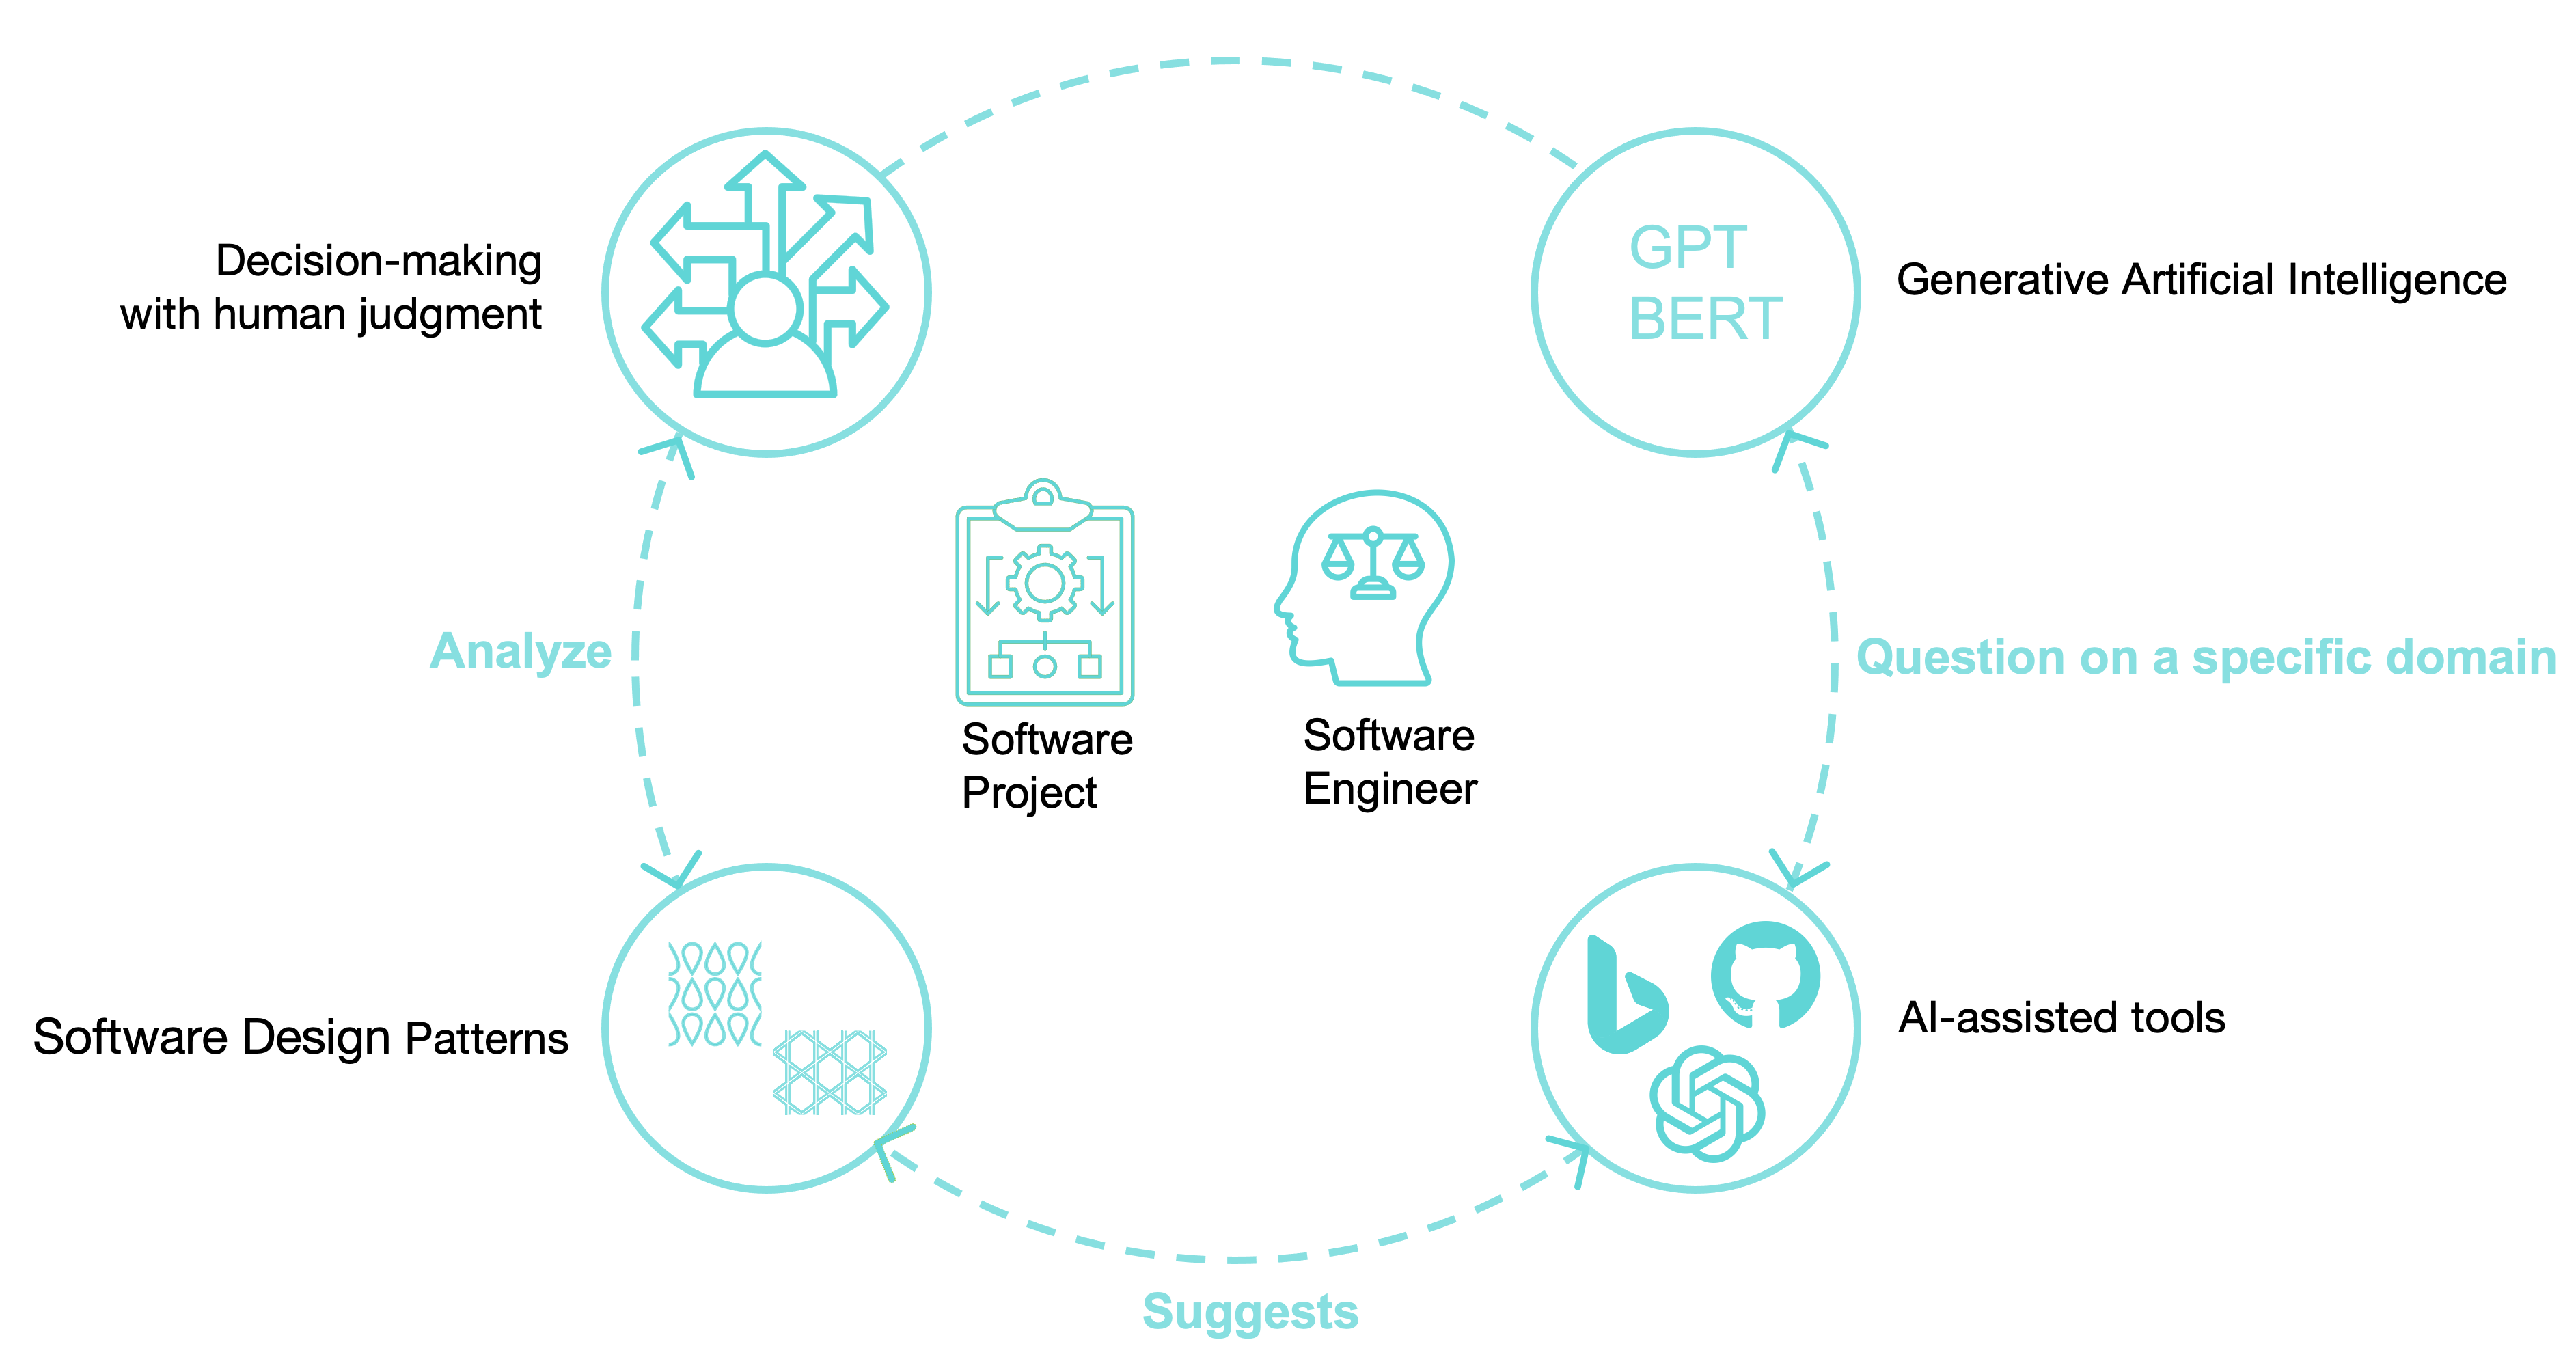
\includegraphics[width=0.80 \textwidth]{figures/context.png}
\objectsource{\objectsourceauthor}
\end{figure}
% End Figure ---------------------------

This collaboration between \ac{GAI Tools} and developers is relatively new, so it is crucial to understand its effectiveness and possible side effects, the nature of interactions, how these tools will be incorporated into the software development cycle, and the perceived benefits of particular interest. Furthermore, assessing whether using such devices leads to improvements or accelerates the software development process is necessary. Thus, detailed assessments of how developers and companies use \ac{GAI Tools} in their software development cycles are essential to incorporate and optimize these new technologies successfully.

\section{Objective}\label{sec:objective} 
\label{section objective}
\begin{quote}
The goal of this dissertation is: \textbf{\textit{Evaluating Generative Artificial Intelligence Tools for assisting architects in software architecture decision-making using prompt patterns sequence.}}
\end{quote}

\section{Research Questions}\label{sec:research-questions}
\begin{quote}
\textbf{\textit{How do generative AI tools, specifically from GPT models, can be used to support software architecture decision-making process?}}

\begin{itemize}
    \item  \textbf{\textit{RQ\textsubscript{1}: What is the efficiency and accuracy of generative AI tools, such as GPT, in solving software design problems?}} -- To answer that question, we performed an exploratory study that used existing questions that asked the right design pattern for a design problem to investigate how generative AI tools perform.
    \item \textbf{\textit{RQ\textsubscript{2}: What approaches can be applied in using generative AI tools to support decision-making in software architecture?}} -- To answer that question, our work is based on existing prompt patterns and uses design science to explore other alternatives. As a result, a new set of prompt patterns and a prompt sequence was proposed.
    \item \textbf{\textit{RQ\textsubscript{3}: What are the perceived benefits and challenges of using the proposed prompt sequence with generative AI tools in the architectural decision-making process from the perspective of software architects?}} -- To answer that question, we applied the prompt sequence in past problems faced by companies and interviewed software architects that participated in the decision process to collect their impressions.   
\end{itemize}

% Answering these research questions will provide a comprehensive view of current AI-assisted tools for design decision-making in software projects and insights into their future directions and opportunities.
\end{quote}

\section{Methodology}\label{sec:methodology}
For this master's project, two parts of research are conducted. The first study will explore using pre-trained generative AI tools to automatically select design patterns in a specific context. This will help us better understand how this new technology behaves when presented with a problem. The second study will use multiple case studies to analyze companies' effectiveness in real-world scenarios.

The literature review played a pivotal role in shaping the direction of our research project, inspiring the approach for both phases of investigation. We gained valuable insights into the field's current state by delving into relevant literature on design decision-making, design patterns, and AI-assisted tools. This comprehensive understanding of the subject helped us identify useful generative AI tools and provided the groundwork for the concept of automatic design pattern selection.

We conducted a preliminary study to determine the effectiveness of AI tools in helping developers make design decisions. Specifically, we utilized ChatGPT to assess its ability to provide accurate answers and ensure that its suggestions included all required elements for a given pattern. Additionally, we tested whether incorrect responses from the AI could potentially mislead developers.

Based on the positive results from our preliminary study, we plan to move forward with multiple case studies in five distinct phases, shown in Figure~\ref{fig-methodology}.

% Inicio Figura1 ---------------------------
\begin{figure}[ht]
\caption{Overview of the methodology adopted for AI-Assisted Design Decision Research.}
\centering
\label{fig-methodology}
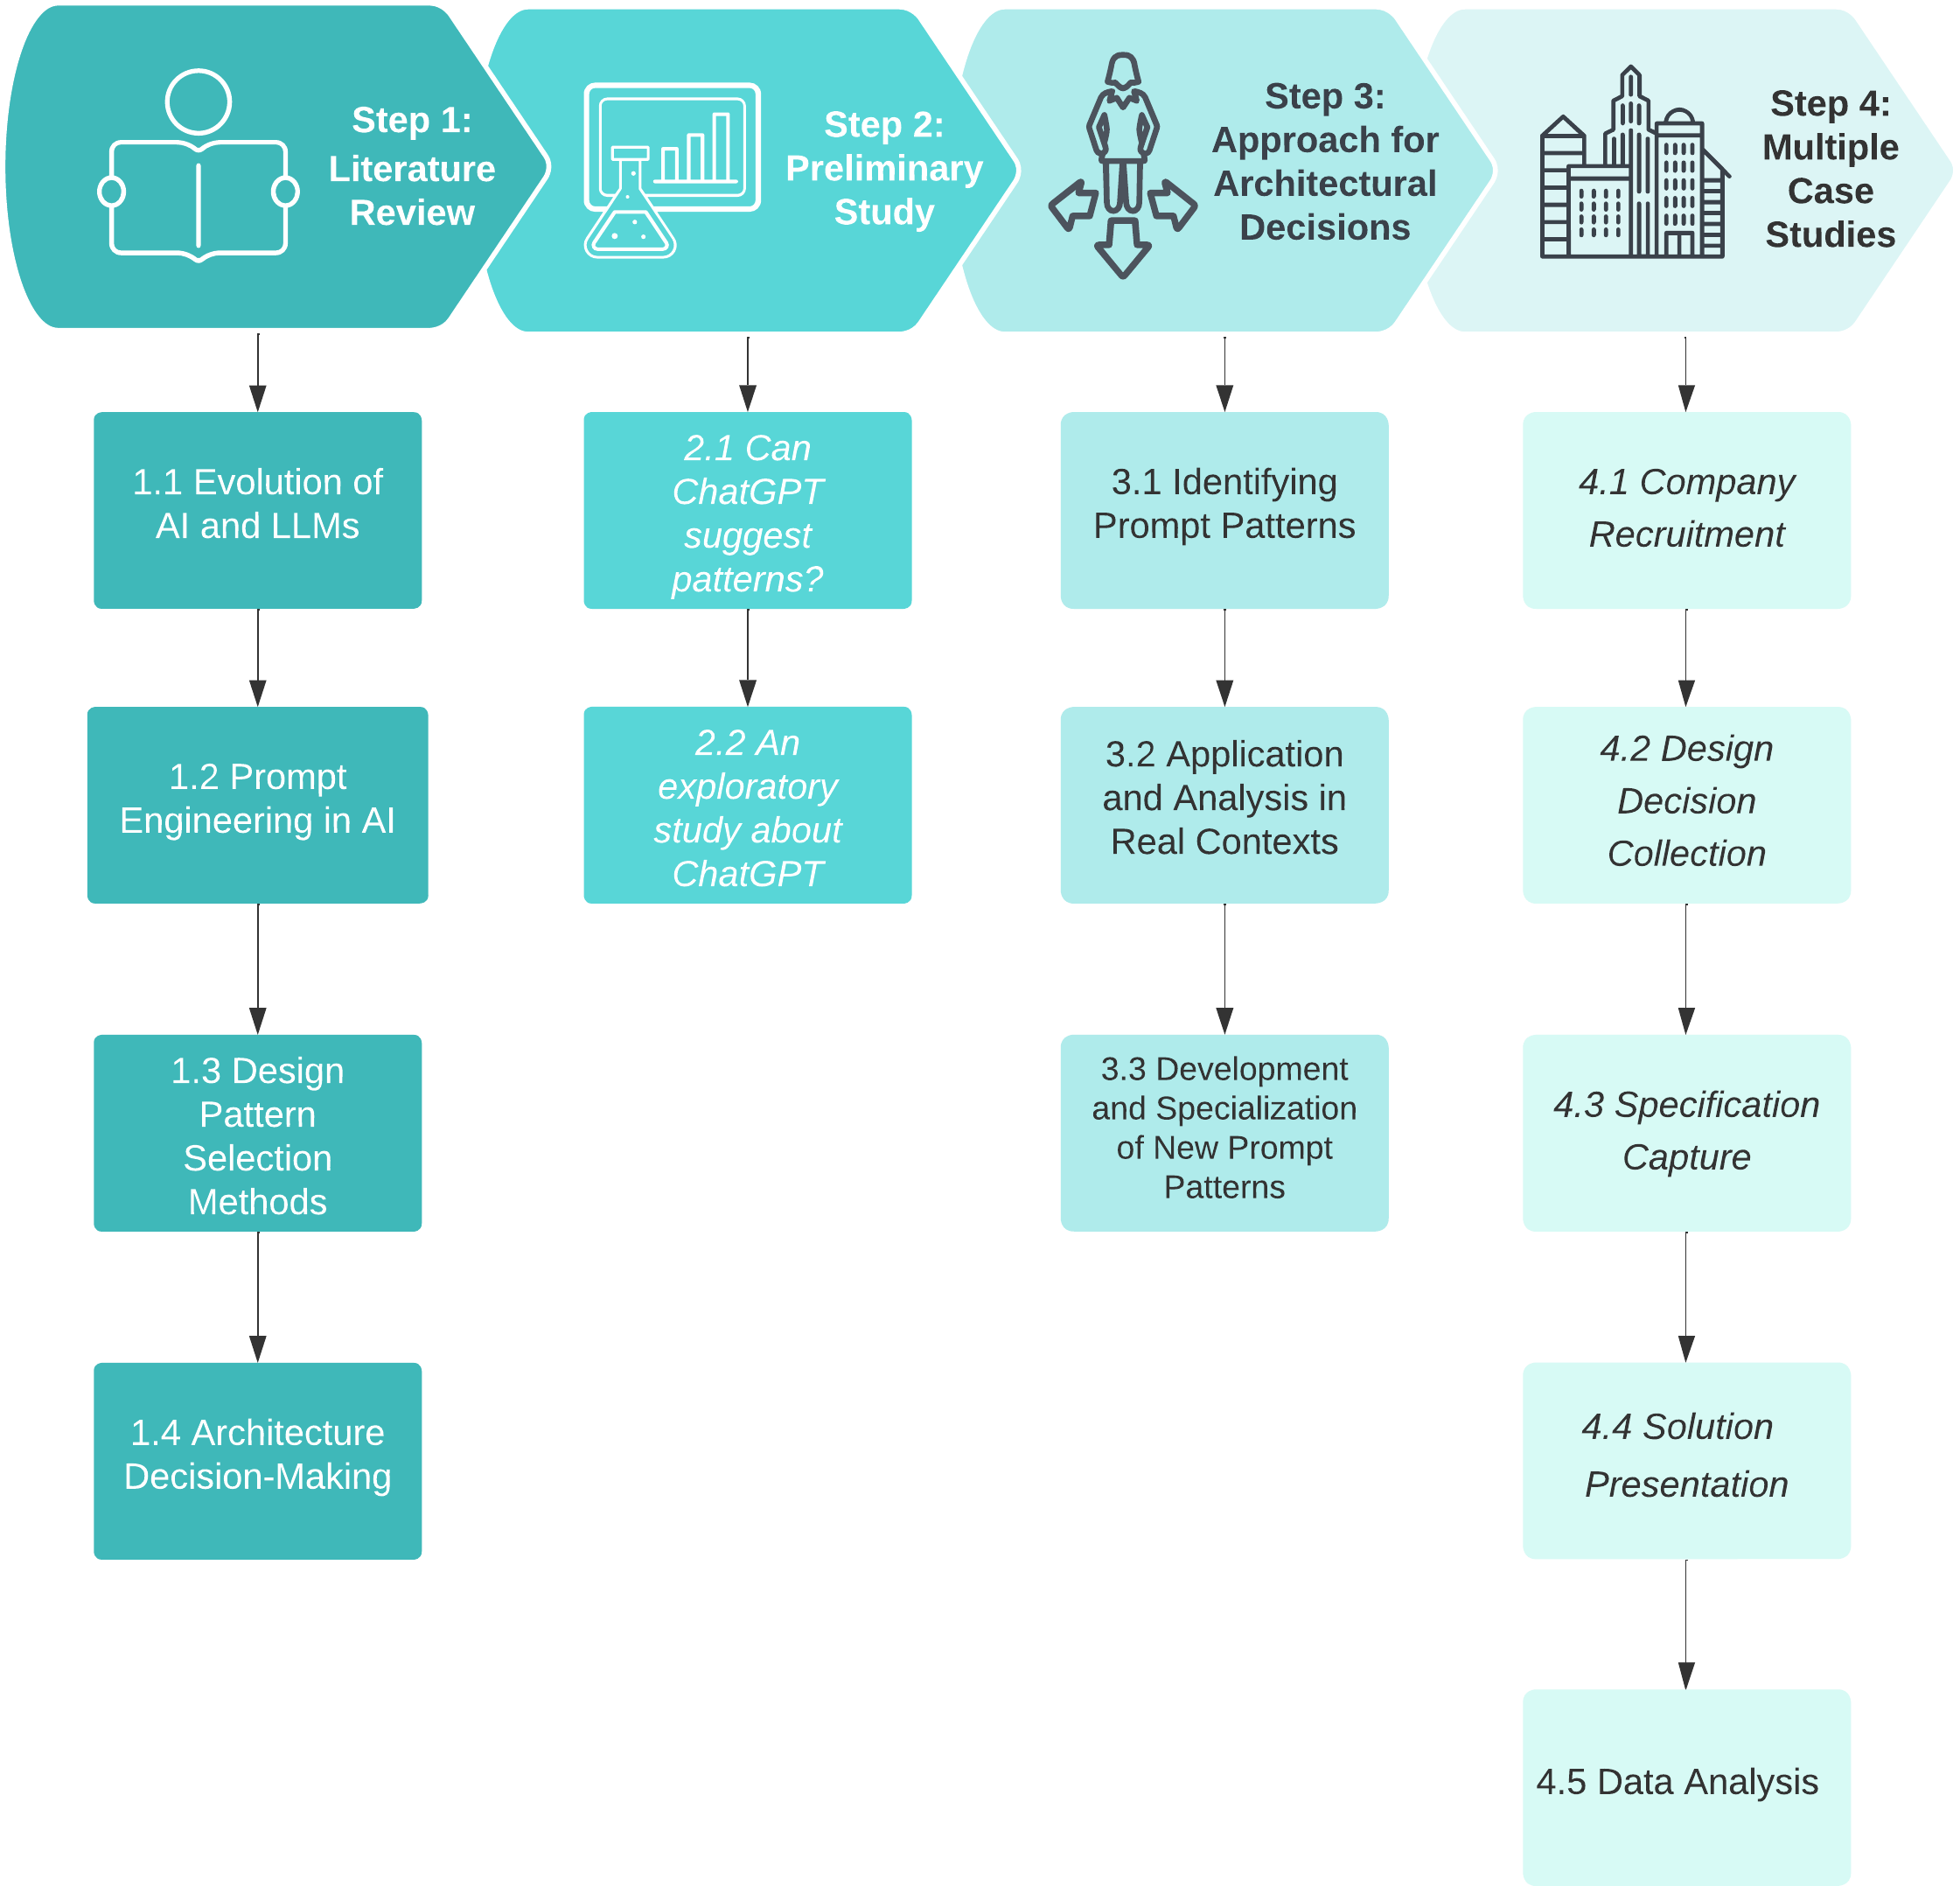
\includegraphics[width=0.90 \textwidth]{figures/current-methodology.png}
\objectsource{\objectsourceauthor}
\end{figure}
% Fim Figura1 ---------------------------


\begin{enumerate}
    
\item \textbf{Recruitment} - in this phase, we aim to select at least three companies to participate in our study. The selection process will prioritize diversity across various businesses, providing a wide range of perspectives and enhancing our results.

\item \textbf{Design Decision Collection} - focused on Collecting Design Decisions We will identify a critical decision related to architecture or software for each participating company. This decision must be an essential and challenging one to test the capabilities of language models accurately. Together with the enterprise's software architect, we will formulate a question encompassing an application scenario and all the significant factors influencing the decision-making process.

\item  \textbf{Specification Capture} - we will Capture Specifications using prompt engineering techniques to formulate questions for three AI tools that use Large Language Models. The responses generated by the language models will be carefully evaluated, and the relevant materials will be prepared for further analysis and presentation.

\item  \textbf{Solution Presentation} - focuses on presenting the solution. Proposed solutions will be presented to the company's architect in an interview format. We will measure the solution's suitability for the system, assessing how the proposed solution could be implemented. This feedback will be invaluable in refining our understanding of the language model's capability and effectiveness in real-world scenarios.
    
\item \textbf{Data Analysis} - we will analyze the data. During this step, we will apply Open Coding qualitative analysis techniques to analyze the three AI tools' responses, collected specifications, and interview feedback on the proposed solution. This rigorous analysis will elucidate patterns, highlight discrepancies, and reveal insights into the usefulness and applicability of language models in architectural and software design decision-making.
\end{enumerate}

\MyParaBold{Advantages of This Approach Methodology:}
\begin{enumerate}
    \item \textbf{Bridging Theoretical Exploration and Practical Application:} This methodology offers insights into how emerging technologies could enhance architectural decision-making by speculatively evaluating the impact of generative AI and prompt patterns on past decisions. This bridges the gap between theory and practice, providing academic and practical value.

    \item \textbf{Dynamic Engagement:} Unlike traditional methodologies that rely heavily on documentation, this approach allows for a more interactive and reflective examination of past decisions, enriching the analysis with hypothetical scenarios that blend real-world experiences with theoretical possibilities.

    \item \textbf{Prompt Patterns Integration:} The focus on AI-generated prompt patterns emphasizes the study's contribution to discussions about integrating emerging technologies into architectural practices. This advances academic understanding and is a practical guide for incorporating new tools into decision-making processes.
    
    \item \textbf{Flexibility and Innovation:} This methodology showcases the flexibility of empirical research methods in software engineering by adapting and combining elements from different approaches to suit specific research objectives, highlighting the potential of empirical research in the field.  
\end{enumerate}



\section{Originality}\label{sec:originality}
The originality of this master's work lies in exploring and evaluating the potential of AI-assisted tools in software design decision-making. Here, the research emphasizes assessing how software development professionals perceive the use of AI tools within the software development cycle; despite the broad integration of AI in various aspects of software engineering, it has yet to be examined thoroughly in this specific context.

This work also stands out for its focus on evaluating unsupervised AI tools, such as ChatGPT, through the preliminary study to design pattern suggestions. Most current pattern selection approaches require specialized training or knowledge. However, the preliminary study approach employs AI tools that do not require such stringent prerequisites. This perspective offers relatively new insight into the field of software engineering.

Furthermore, this research analyses the interaction of AI and human experience, where both elements combine to create a unique collaborative approach to decision-making in software design. This work promises to shed light on the potential synergies and challenges arising from this combination, a facet of software development that has not been explored in great detail before.

The empirical nature of this research provides an additional layer of originality as it sets out to offer valuable evidence on the productivity of software architects when they engage with AI tools. Considering the relative scarcity of empirical data in the domain of AI in software design decision-making, its study can fill a significant gap.

Finally, its focus on understanding the sociotechnical aspects of AI architecture brings perspective to the challenges of automated and collaborative software engineering. By assigning the same importance to software design and development's social and technical aspects, this work is expected to offer critical insights that need to be more widely addressed in the existing literature.

\section{Relevance}\label{sec:relevance}
\textbf{From an industry perspective}, applying AI-assisted tools for decision-making in software projects promises significant improvements in the software development process. By identifying and recommending appropriate design patterns, software developers can save crucial time and resources, streamlining their workflows and ensuring shorter development cycles and accelerated time-to-market for software products.

This efficiency gain is supported by the subsequent improvement in code quality that these tools promise. Design patterns are vital to ensure code modularity, maintainability, scalability, critical software quality, and robust components. By helping developers select the most suitable patterns for specific scenarios, these AI-assisted tools not only help improve the initial quality of the software product but also simplify its long-term maintenance. A review of the relevant literature and the results of preliminary studies indicate that pattern selection aided by pre-trained generative AI can outperform conventional selection methods in accuracy and efficiency.

Additionally, these tools are invaluable in supporting junior developers. With limited experience in software design, these individuals can significantly benefit from the detailed explanations and solutions offered by AI-assisted tools. Such assistance can accelerate learning, allowing these developers to make informed design decisions early in their careers.

Communication can be more challenging when working remotely due to the lack of face-to-face interaction and possible time zone differences. This can make it difficult to discuss and design decision-making. AI-assisted tools can facilitate this process by recommending appropriate decisions, reducing the need for extensive deliberations, and increasing efficiency.

\textbf{From an academic perspective}.The project bridges the gap between academic theory and practical application, providing valuable insights through real-life exercises and case studies. These insights can be implemented directly into software development to improve decision-making processes. The study also identifies areas where AI tools need improvement, allowing researchers and developers to focus on improving these tools. This research may inspire exploration of other fields where AI can be utilized for complex decision-making tasks like a prompt engineer, leading to broader use of this technology.

\section{Organization}\label{sec:organization}
\begin{quote}
The rest of this document is structured as follows: 
\end{quote}

\begin{itemize}
    
\item Chapter~\ref{ch:literature-review} - Literature Review: This chapter provides valuable information about an overview of Artificial Intelligence, Prompt Engineering for Generative, Few-Shot Learning, and various approaches to selecting design patterns, revealing a gap in the absence of generative AIs to discover such design patterns.
 
 \item Chapter~\ref{ch:preliminar-study} - The Preliminary Study: This chapter uses pre-trained AI tools to automatically select design patterns in a specific context. It assesses the accuracy of AI-generated responses and their potential to guide developers effectively.

\end{itemize}